\section{Generate Test Cases}
\marginnote{Most books talk about correct solutions only.  Few books
  talk about incorrect methods and why they are wrong.  This book
  takes a different approach: we assume that mistakes are unavoidable
  and explain strategies to prevent, detect, and correct the mistakes.
}

Lacking test cases of known properties is one common problem in
developing software for machine learning.  The purpose of machine
learning is to recognize unknown patterns in data; thus, we do not
know the patterns in advance.  How can we know that the programs are
correct?  If we do not know that the programs are correct, how do we
know the patterns discovered by the programs are correct?  Two methods
are commonly used:
\begin{enumerate}
\item Creating simple test cases manually with known properties.

\item Adopting widely used test cases whose properties have already
  been studied.
\end{enumerate}
The first methods is restricted to only very small test cases that are
unlikely to have sophisticated patterns needed to test computer
programs.  The second methods, in contrast, may sophisticated patterns
but the data may be too complex for identify problems in the programs.

\index{test case generator}

\marginnote{When developing programs, it is common to test using cases
  of known properties generated by computer programs (called {\it test
    case generators} in this book).  }

This book suggests the third approach: write another program (or
several programs) to generate the test cases of known properties.
More specifically, for this problem, we can write a program that
generates $n$ data points in $k$ clusters ($n > k$).  Since the data
points are generated intentionally, it is easy to test whether a
k-mean program is correct.

Writing a test case generator, however, is not trivial because the
generator has to consider many different possible properties of data
collected in different scenarios. It is likely that different
generators would be needed in different scenarios. This section
explains one generator. Readers may need to change this generator to
meet different needs.  This generator has the following input
arguments:\marginnote{Determining the inputs is an important part of
  designing software.}

\begin{itemize}
\item Number of dimension ($p$ in the explanation).  Each data point
  is a $p$-dimensional vector. The minimum value is 1.

\item Number of clusters (called $m$ in this program).  This program
  restricts that $m$ must be greater than two.  The program
  intentionally uses a different symbol ($m$) to distinguish from the
  value $k$ given to the clustering program to be tested.

\item Minimum numbers of data points per cluster (called $q$ in this
  program).  This program restricts that $q$ must be at least three.

\item Maximum numbers of data points per cluster (called $r$ in this
  program). Obviously, $r$ must be greater than $q$.

\end{itemize}  

All these arguments are positive integers.  The programs in this
chapter handles integers only because floating-point numbers have
limited precision and sometimes give surprising results.  The number of
data points $n$ is between $m q$ and $m r$.
\marginnote{Chapter~\ref{ch:floatingpoint} has more details about how
  the limited precision may affect results in analysis.}  This program
generates two output files: {\tt data.txt} and {\tt cluster.txt}.  The
first file has $n$ lines and each line has $p$ integers.  The second
file also has $n$ lines; each line has the same $p$ integers,
following by one integer between $0$ and $m - 1$ to indicate which
cluster this line belongs to.

This program is pretty simple: it divides $(-1000m, 1000m)$ in each
dimension into $m$ regions. The centroids of two adjacent regions are
separated by 2000 in each dimension.  The data points of a particular
cluster are scattered within 200 around the cluster's centroid.  The
following is the test case generator.

\resetlinenumber[1]
\linenumbers
\begin{tt}
  \lstinputlisting{\progpath/unsupervised/kmean/testgen/main.py}
\end{tt}
\nolinenumbers

\resetlinenumber[1]
\linenumbers
\begin{tt}
  \lstinputlisting{\progpath/unsupervised/kmean/testgen/testgen.py}
\end{tt}
\nolinenumbers

This is a sample output of the program using the default values for
the arguments: $(p, m, q, r) = (2, 3, 3, 5)$.
This is an example of the output {\tt data.txt}.

\resetlinenumber[1]
\linenumbers
\begin{tt}
  \lstinputlisting{\kmeanpath/data/data1.txt}
\end{tt}
\nolinenumbers

This is an example of the corresponding {\tt cluster.txt}.

\resetlinenumber[1]
\linenumbers
\begin{tt}
  \lstinputlisting{\kmeanpath/data/cluster1.txt}
\end{tt}
\nolinenumbers

\section{Visualize Data}

\index{high-dimensional}

This chapter presents a program that can visualize data up to three
dimensions.  The purpose of this visualization is to help inspect
whether the data produced by the test generator is indeed clustered
into several regions.

\resetlinenumber[1]
\linenumbers
\begin{tt}
  \lstinputlisting{\progpath/unsupervised/kmean/testgen/visualize.py}
\end{tt}
\nolinenumbers

\marginnote{It is common that the data of interest is {\it
    high-dimensional} and visualizing the data would be difficult.  }

The following figures show the generated data in one, two, and three
dimensions.  The figures are drawn using {\tt visualize.py}.


\clearpage

\begin{figure}[h] \centering
 \subfigure[]
{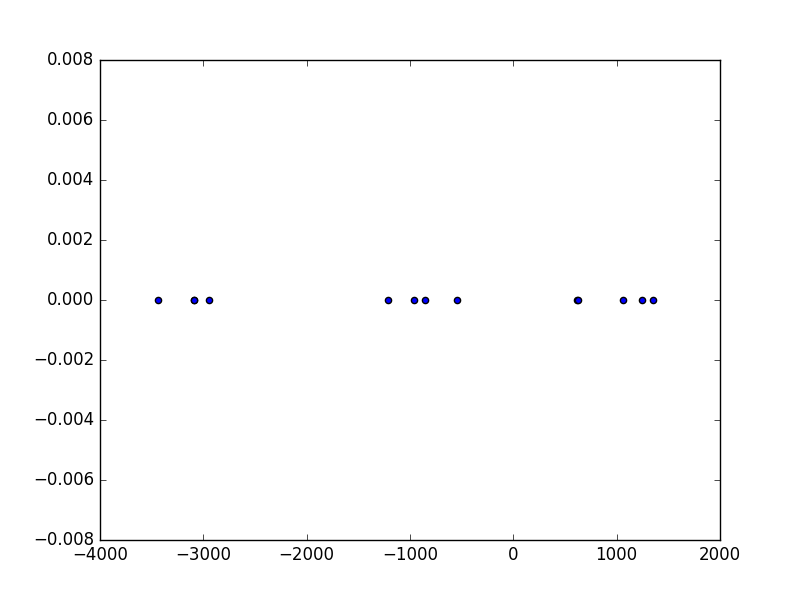
\includegraphics[width=3in]{\kmeanpath/figures/figure1.png}}
  \subfigure[]
{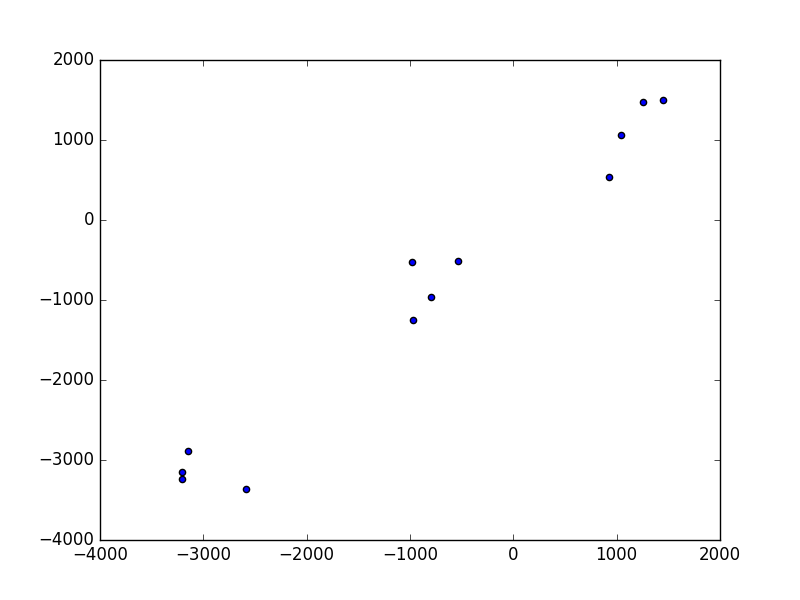
\includegraphics[width=3in]{\kmeanpath/figures/figure2.png}}
  \subfigure[]
{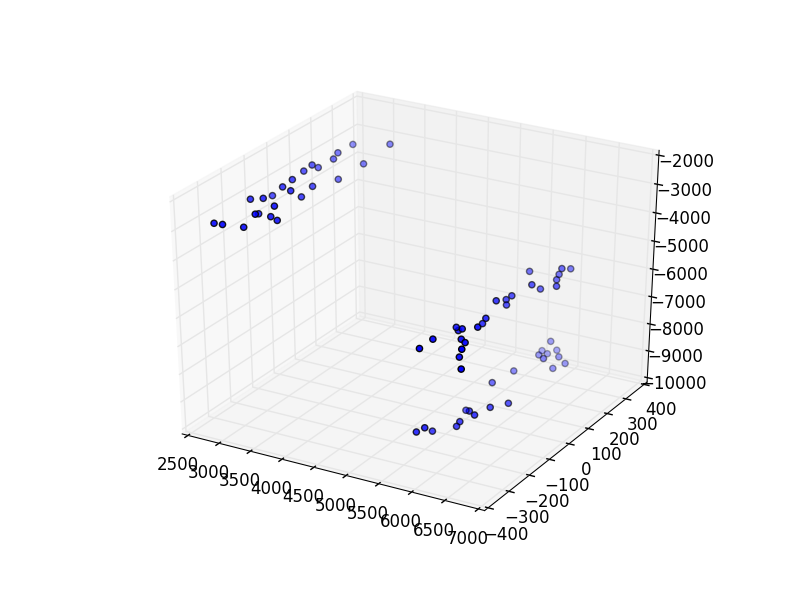
\includegraphics[width=3in]{\kmeanpath/figures/figure3.png}}
\caption{Visualize the generated test cases in (a) one, (b) two, and
  (c) three Dimensions. }
\label{fig:kmean:visualize}
\end{figure}

\clearpage

\section{K-Mean Algorithm Implementation}

Now is the time to show how the {\it K-Mean} algorithm can be
implemented. The implementation pretty much reflects the algorithm
described on Page~\pageref{algorithm:kmean}.

\resetlinenumber[1]
\linenumbers
\begin{tt}
  \lstinputlisting{\progpath/unsupervised/kmean/solution/main.py}
\end{tt}
\nolinenumbers

\resetlinenumber[1]
\linenumbers
\begin{tt}
  \lstinputlisting{\progpath/unsupervised/kmean/solution/kmean.py}
\end{tt}
\nolinenumbers

\resetlinenumber[1]
\linenumbers
\begin{tt}
  \lstinputlisting{\progpath/unsupervised/kmean/solution/datapoint.py}
\end{tt}
\nolinenumbers

\resetlinenumber[1]
\linenumbers
\begin{tt}
  \lstinputlisting{\progpath/unsupervised/kmean/solution/centroid.py}
\end{tt}
\nolinenumbers


Does this program work? Let's try a few examples. Suppose this
is the input {\tt data.txt}. There are four clusters.

\resetlinenumber[1]
\linenumbers
\begin{tt}
  \lstinputlisting{\kmeanpath/data/data2.txt}
\end{tt}
\nolinenumbers

This is the corresponding {\tt cluster.txt}
and the result when $k$ is 4. They are put side-by-side
for easy comparison.

{\bf GKT, why there are no line numbers below?}

\begin{minipage}[t]{0.4\textwidth}
\resetlinenumber[1]
\linenumbers
\begin{tt}
  \lstinputlisting{\kmeanpath/data/cluster2.txt}
\end{tt}
\nolinenumbers
\end{minipage}
\begin{minipage}[t]{0.4\textwidth}
\resetlinenumber[1]
\linenumbers
\begin{tt}
  \lstinputlisting{\kmeanpath/data/result2.txt}
\end{tt}
\nolinenumbers
\end{minipage}

This example shows that the {\it k-mean} clustering works great: it
successful divides the data into four clusters in the same way as the
data is generated, except that cluster labels may be different; for
example, the original cluster 1 is called cluster 3.

This is another example with 5 clusters

\begin{minipage}[t]{0.4\textwidth}
\resetlinenumber[1]
\linenumbers
\begin{tt}
  \lstinputlisting{\kmeanpath/data/cluster4.txt}
\end{tt}
\nolinenumbers
\end{minipage}
\begin{minipage}[t]{0.4\textwidth}
\resetlinenumber[1]
\linenumbers
\begin{tt}
  \lstinputlisting{\kmeanpath/data/result4.txt}
\end{tt}
\nolinenumbers
\end{minipage}

This program uses different symbols for the clusters

\resetlinenumber[1]
\linenumbers
\begin{tt}
  \lstinputlisting{\progpath/unsupervised/kmean/solution/visualize.py}
\end{tt}
\nolinenumbers


\clearpage

\begin{figure}[h] \centering
{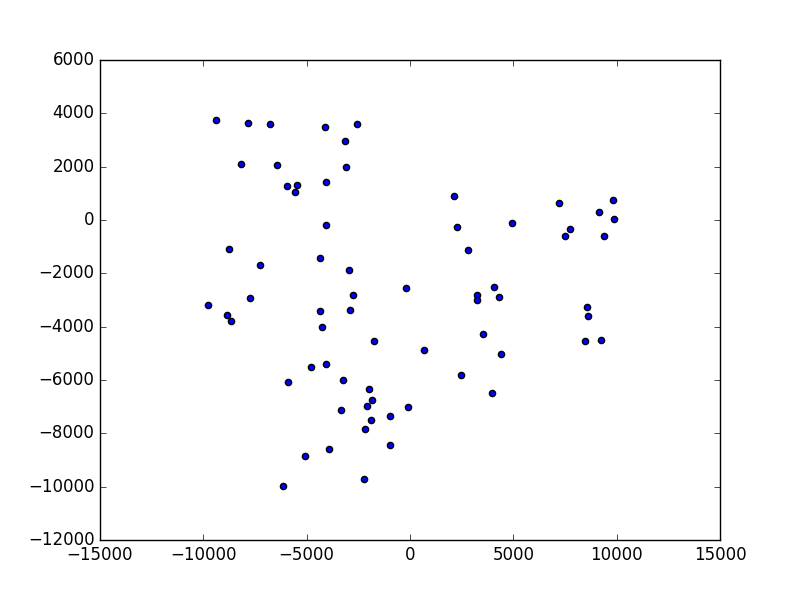
\includegraphics[width=4in]{\kmeanpath/figures/figure4.png}}
\caption{The figure visualizes the five clusters. Each cluster
uses a unique symbol.}
\label{fig:kmean:clusters}
\end{figure}

\clearpage

So far the data is generated by the test case generator and the data
points are clearly clustered without any overlap.  Now, let's see how
the {\it k-mean} algorithm behaves when the data is not as ideal as
earlier.  We are going to run the test case generator again but with
the {\tt -t} argument, allowing clusters to overlap.  We will also
choose 5 clusters using the {\tt -m} argument.  Each cluster has
at least 10 data points and at most 15 points.
Let's visualize the data:
% the data and clusters are stored in
% \kmeanpath/data/data5.txt and
% \kmeanpath/data/cluster5.txt and


\begin{figure}[h] \centering
  \subfigure[]
  {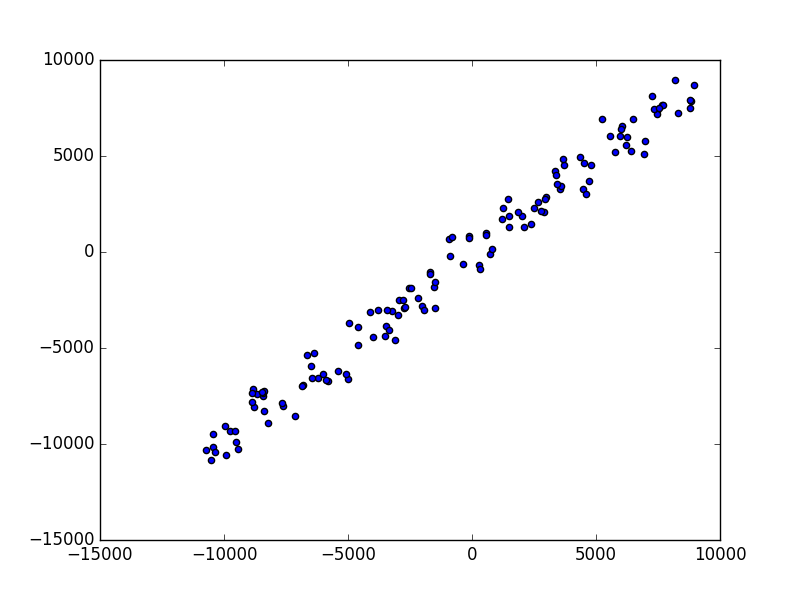
\includegraphics[width=4in]{\kmeanpath/figures/figure5.png}}
  \subfigure[]
{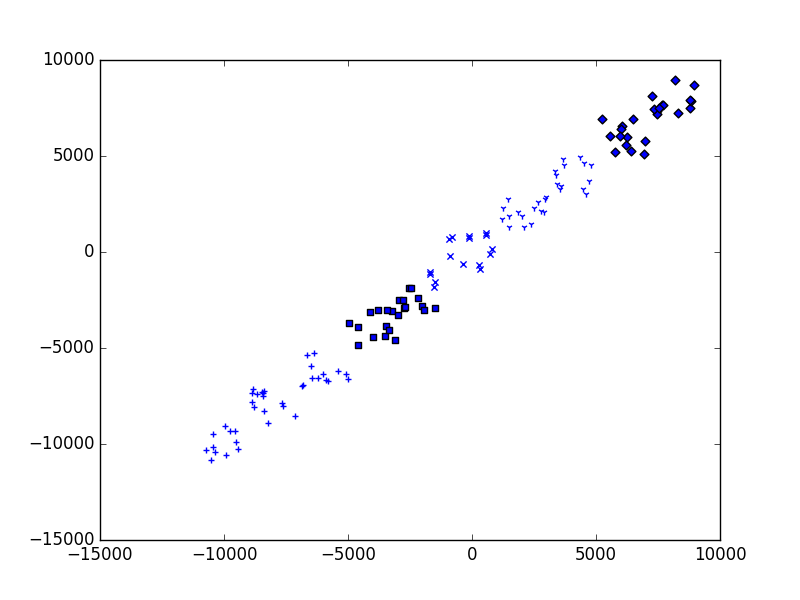
\includegraphics[width=4in]{\kmeanpath/figures/figure6.png}}
\caption{(a) Data generated using {\tt -t -m 10 -q 10 -r 15}.
(b) K-Mean result using 5 clusters (i.e., $k$ is 5). }
\label{fig:kmean:cluster5}
\end{figure}

\section{Understand Non-Deterministic Behavior of K-Mean}

This is great, right? Let us run the clustering program again.

\resetlinenumber[1]
\linenumbers
\begin{tt}
  \lstinputlisting{\kmeanpath/data/result3.txt}
\end{tt}
\nolinenumbers

There is a problem. Cluster 2 has 9 data points and cluster 3 has
only one data point. How can this program produces different
results even though the input data is the same?  A simple
answer is that this program is {\it non-deterministic}.
The reason this program is non-deterministic is this line in
{\tt kmean.py}:

\index{non-deterministic}
\begin{verbatim}
        clu = random.randint(0, kval - 1)
\end{verbatim}

\index{random number generator}

It assigns each data point to a cluster between $0$ and $k-1$
randomly.  It is possible that two or more data points in the same
cluster ( they are in the same cluster by the test generator) are
assigned to different clusters.

Python (and most programming languages) has a {\it random number
  generator}.  It generates random numbers. What does this mean?  It
means that it would be difficult to predict the next number after
observing a sequence of numbers.  
Let us consider several examples. This is a simply program calling
Python's {\tt random.randint}. 

\resetlinenumber[1]
\linenumbers
\begin{tt}
  \lstinputlisting{\progpath/unsupervised/kmean/random/sequence1.py}
\end{tt}
\nolinenumbers

The following shows the results
executing the program three times; each column is the result of
executing the program once.

\begin{tabular}{p{1in}p{1in}p{1in}}
\begin{tt}
  \lstinputlisting{\kmeanpath/data/sequence1.txt}
\end{tt}
&
\begin{tt}
  \lstinputlisting{\kmeanpath/data/sequence2.txt}
\end{tt}

&
\begin{tt}
  \lstinputlisting{\kmeanpath/data/sequence3.txt}
\end{tt}

\end{tabular}

Reading top to bottom inside each column, it is difficult to predict
the next number from the numbers that have already been seen.
Comparing different columns, the sequences are different.

\index{random number generator!seed}
Python allows programmers to set  the {\it seed} of the random number generator.
If the same seed is same, the same sequence of numbers is generated.
In other words, the sequence becomes {\it deterministic}.  The following program
always generates the same sequence of numbers.


\resetlinenumber[1]
\linenumbers
\begin{tt}
  \lstinputlisting{\progpath/unsupervised/kmean/random/sequence2.py}
\end{tt}
\nolinenumbers

\index{security key}

The words {\it random} and {\it non-deterministic} are often confused.
Random means it is difficult to predict in advance.  {\it
  Non-deterministic} means that if the same program runs again with
the same inputs, the results may be different.  It is possible to have
a deterministic sequence of random numbers, like the ones generated by
{\tt sequence2.py}.  The sequence is deterministic because running the
program again generates the same sequence. The sequence is random
because knowing the generated numbers cannot predict the future
numbers.

\index{random number generator!seed}


A common way of varying the seed is using the microsecond of the
current time in the following way:

\begin{verbatim}
        random.seed(datetime.datetime.now().microsecond)
\end{verbatim}

\marginnote{Be careful using time as random number seeds for keys in
  security programs.  Using microseconds restrict the possible keys to
  only 0 and 999999.  This small range of seeds weakens security
  because there are only one million possibilities.}

